\documentclass[12pt,a4paper]{report}
\usepackage[utf8]{inputenc}
\usepackage[T1]{fontenc}
\usepackage[ngerman]{babel}
\usepackage{graphicx}
\usepackage{hyperref}
\usepackage{amsmath}
\usepackage{amssymb}
\usepackage{geometry}
\usepackage{setspace}
\usepackage{xcolor}
\usepackage{float}
\usepackage{listings}
\usepackage{helvet}
\usepackage{parskip}
\usepackage{titlesec}
\usepackage{caption}



\definecolor{codegreen}{rgb}{0,0.6,0}
\definecolor{codegray}{rgb}{0.5,0.5,0.5}
\definecolor{codepurple}{rgb}{0.58,0,0.82}
\definecolor{backcolour}{rgb}{0.95,0.95,0.92}

\lstdefinestyle{mystyle}{
    backgroundcolor=\color{backcolour},   
    commentstyle=\color{codegreen},
    keywordstyle=\color{magenta},
    numberstyle=\tiny\color{codegray},
    stringstyle=\color{codepurple},
    basicstyle=\ttfamily\footnotesize,
    breakatwhitespace=false,         
    breaklines=true,                 
    captionpos=b,                    
    keepspaces=true,                 
    numbers=left,                    
    numbersep=5pt,                  
    showspaces=false,                
    showstringspaces=false,
    showtabs=false,                  
    tabsize=2
}

\lstset{style=mystyle}

\geometry{a4paper, margin=0.7in}
% Zeilenabstand
\onehalfspacing

\begin{document}

\newpage
\section{Einrichtung des Jetson Orin Nano}
\subsection{Firmware aktualisieren}
Ihr Jetson Orin Nano Developer Kit ist möglicherweise bereits bereit, JetPack 6 auszuführen, da die neueste Firmware (Jetson UEFI Firmware auf QSPI-NOR Flash-Speicher) ab Werk geflasht wurde. Falls dies nicht der Fall ist, müssen Sie auf die neueste Firmware aktualisieren.

Sie können nun die neueste Firmware auf Jetson aktualisieren, ohne einen Host-Ubuntu-PC 
zu benötigen: Befolgen Sie die Schritte auf dieser \textcolor{blue}{\href{https://www.jetson-ai-lab.com/initial_setup_jon.html}{Seite}}, 
um zu überprüfen, ob Ihr Jetson Orin Nano Developer Kit die neueste Firmware hat, 
und aktualisieren Sie diese mit einer SD-Karte, die JetPack 5 enthält.

Folgen Sie den Anweisungen \textcolor{blue}{\href{https://www.jetson-ai-lab.com/initial_setup_jon.html}{hier}}.

Sobald Sie bestätigt haben, dass Ihr Jetson Orin Nano Developer Kit die neueste 
Firmware hat, die JetPack 6 ausführen kann, fahren Sie mit dem nächsten Schritt fort.
\clearpage

\subsection{Image auf die microSD-Karte schreiben}

Um Ihr Jetson Orin Nano Developer Kit einzurichten, müssen Sie die microSD-Karte 
mit dem richtigen Image vorbereiten. Folgen Sie diesen Schritten:

\subsection{Das Jetson Orin Nano Developer Kit-Image herunterladen}
\begin{itemize}
    \item Besuchen Sie das \href{https://developer.nvidia.com/embedded/downloads}{Jetson Download Center} 
    und laden Sie das neueste SD-Karten-Image herunter.
    \item Die heruntergeladene Datei liegt normalerweise im \texttt{.zip}-Format vor. 
    Entpacken Sie die Datei, um die \texttt{.img}-Datei zu erhalten.
\end{itemize}

\subsection{microSD-Karte in den Host-Computer einlegen}
\begin{itemize}
    \item Verwenden Sie einen microSD-Kartenleser, um die Karte in Ihren Computer einzulegen.
    \item Stellen Sie sicher, dass die microSD-Karte von Ihrem Betriebssystem erkannt wird.
\end{itemize}

\subsection{Nutzen Sie SD Card Formatter, um die SD Karte zu formatieren.}
\begin{figure}[h!]
    \centering
    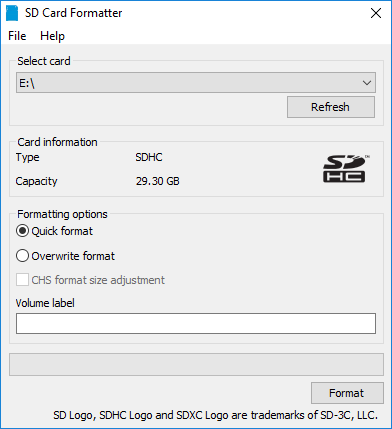
\includegraphics[width=0.6\textwidth ]{Bilder/SD_Card_Formatter.png}
    \caption{SD Card Formatter}
\end{figure}

\begin{itemize}
    \item Laden und führen Sie die \textcolor{blue}{\href{https://www.sdcard.org/downloads/formatter/sd-memory-card-formatter-for-windows-download/}{SD Memory Card Formatter for Windows}} aus.
    \item Wählen Sie das Kartenlaufwerk aus.
    \item Wählen Sie``Schnellformatierung''.
    \item Lassen Sie ``Volume-Label'' leer.
    \item Klicken Sie auf ``Formatieren'', um mit dem Formatieren zu beginnen, und bestätigen Sie mit ``Ja'' im Warn-Dialog.
\end{itemize}
\subsection{Image auf die microSD-Karte schreiben}
\begin{itemize}
    \item Nutzen Sie ein Tool wie Balena Etcher, das für Windows, Mac und Linux verfügbar ist.
\end{itemize}

\textbf{Schritte mit Balena Etcher:}
\begin{enumerate}
    \item Installieren und öffnen Sie \textcolor{blue}{\href{https://etcher.balena.io/}{Balena Etcher.}}
    \begin{figure}[h!]
        \centering
        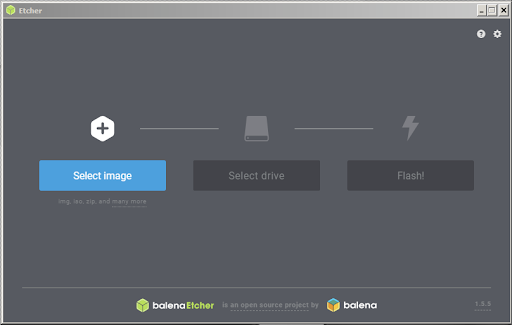
\includegraphics[width=0.6\textwidth ]{Bilder/Etcher.png}
        \caption{Balena Etcher}
    \end{figure}
    \item Wählen Sie die entpackte \texttt{.img}-Datei aus.
    \item Wählen Sie die microSD-Karte als Zielgerät aus.
    \begin{figure}[h!]
        \centering
        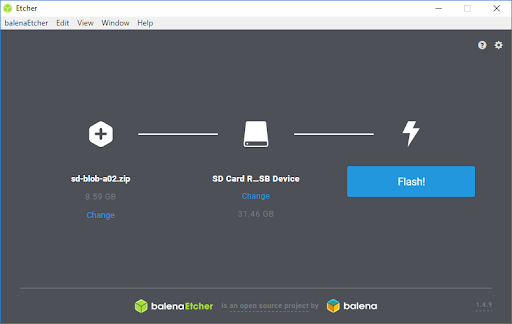
\includegraphics[width=0.6\textwidth ]{Bilder/Etcher_Select_Drive.png}
        \caption{Balena Etcher - Wählen Sie das Zielgerät aus}
    \end{figure}
    \item Klicken Sie auf die Schaltfläche \textquotedblleft Flash\textquotedblright, um das Image auf die Karte zu schreiben.
\end{enumerate}

\subsection{Image überprüfen}
\begin{itemize}
    \item Balena Etcher überprüft automatisch die geschriebenen Daten.
    \item Wenn die Überprüfung fehlschlägt, wiederholen Sie den Flash-Vorgang oder verwenden Sie eine andere microSD-Karte.
\end{itemize}

\subsection{MicroSD-Karte sicher entfernen}
\begin{itemize}
    \item Werfen Sie die microSD-Karte sicher aus, um Datenbeschädigungen zu vermeiden.
\end{itemize}
\clearpage

\section{Flashen und starten}
\subsection{Verbindungen herstellen}
\begin{itemize}
    \item microSD-Karte einlegen: Setzen Sie die vorbereitete microSD-Karte ein.
    \item Peripheriegeräte anschließen: USB-Tastatur, Maus und Monitor.
    \item Netzwerkverbindung herstellen: Ethernet-Kabel anschließen.
    \item Stromversorgung anschließen: 19V-Netzteil mit dem DC-Eingang verbinden.
\end{itemize}
\begin{figure}[h!]
    \centering
    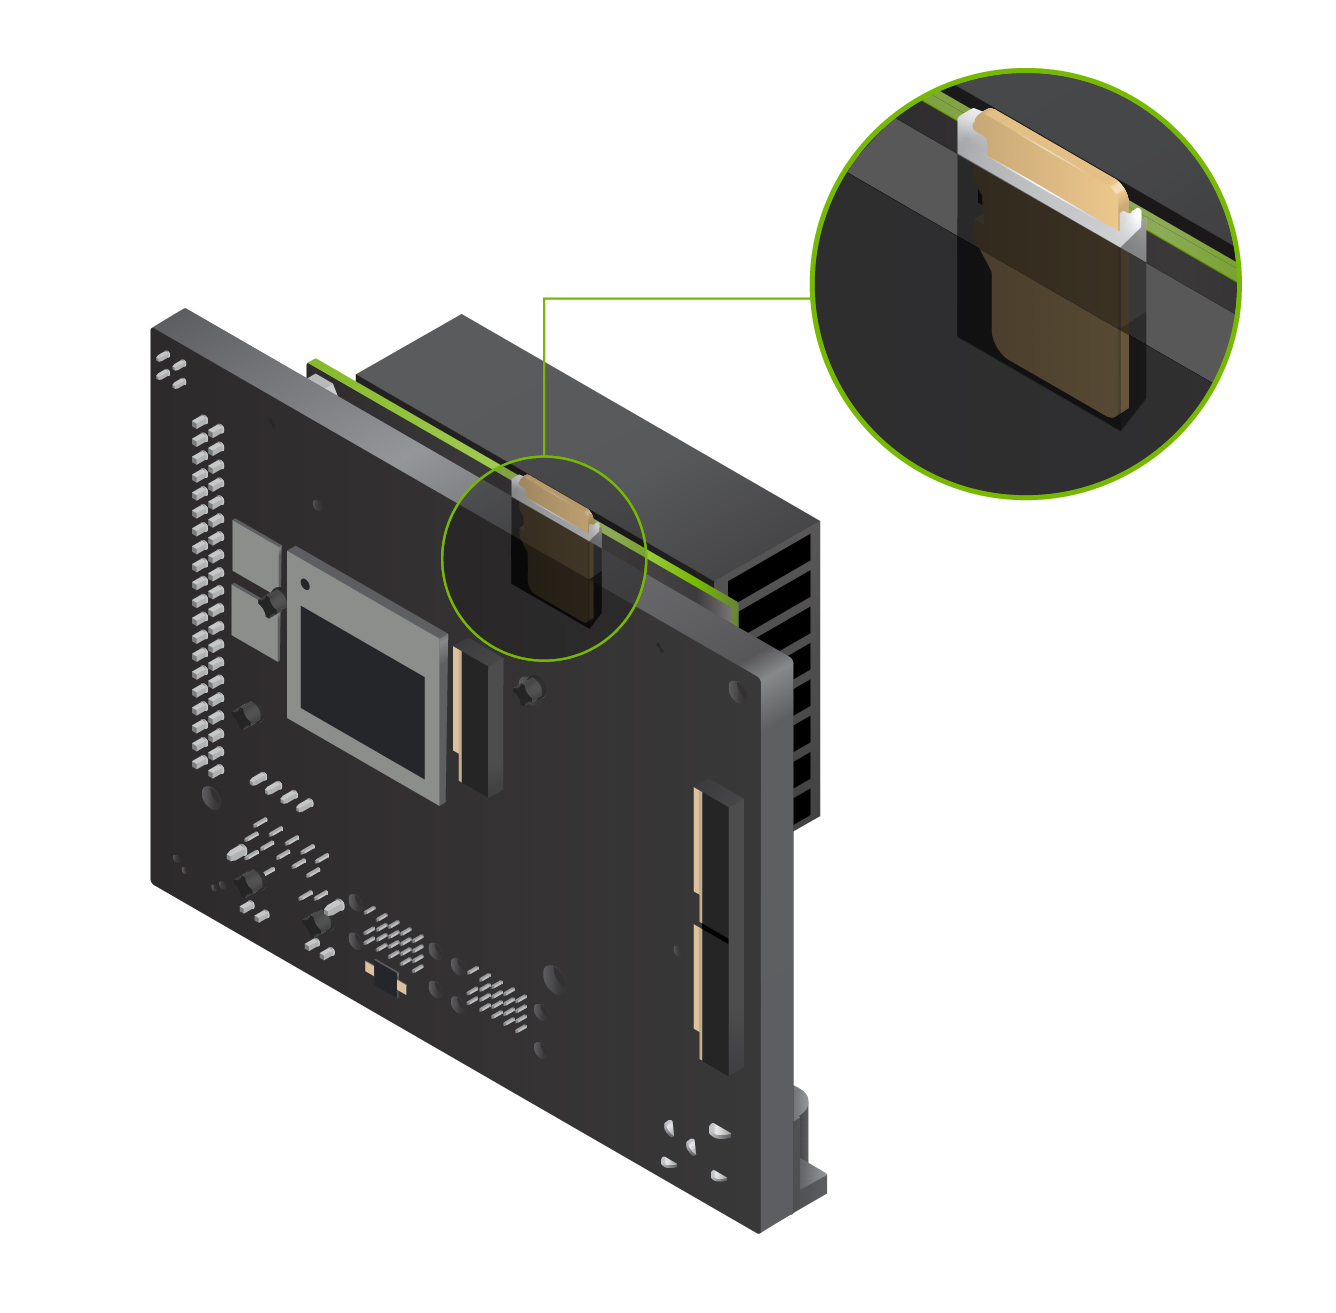
\includegraphics[width=0.8\textwidth ]{Bilder/jetson-orin-nano-dev-kit-sd-slot.jpg}
    \caption{Jetson Orin Nano Developer Kit SD-Kartensteckplatz}
\end{figure}
\clearpage

\subsection{System starten}
Eine grüne LED neben dem USB-C-Anschluss leuchtet auf, sobald das Developer Kit eingeschaltet wird. Beim ersten Bootvorgang führt Sie das Jetson Orin Nano Developer Kit durch die ersten Einrichtungsschritte, darunter:
\begin{itemize}
    \item Überprüfung und Akzeptanz der NVIDIA Jetson Software-EULA
    \item Auswahl der Systemsprache, Tastaturlayouts und Zeitzone
    \item Verbindung mit dem drahtlosen Netzwerk
    \item Erstellen eines Benutzernamens, Passworts und Computernamens
    \item Anmeldung
\end{itemize}

\subsection{Nach dem Login}
Sie werden das folgendes Sehen.
\begin{figure}[h!]
    \centering
    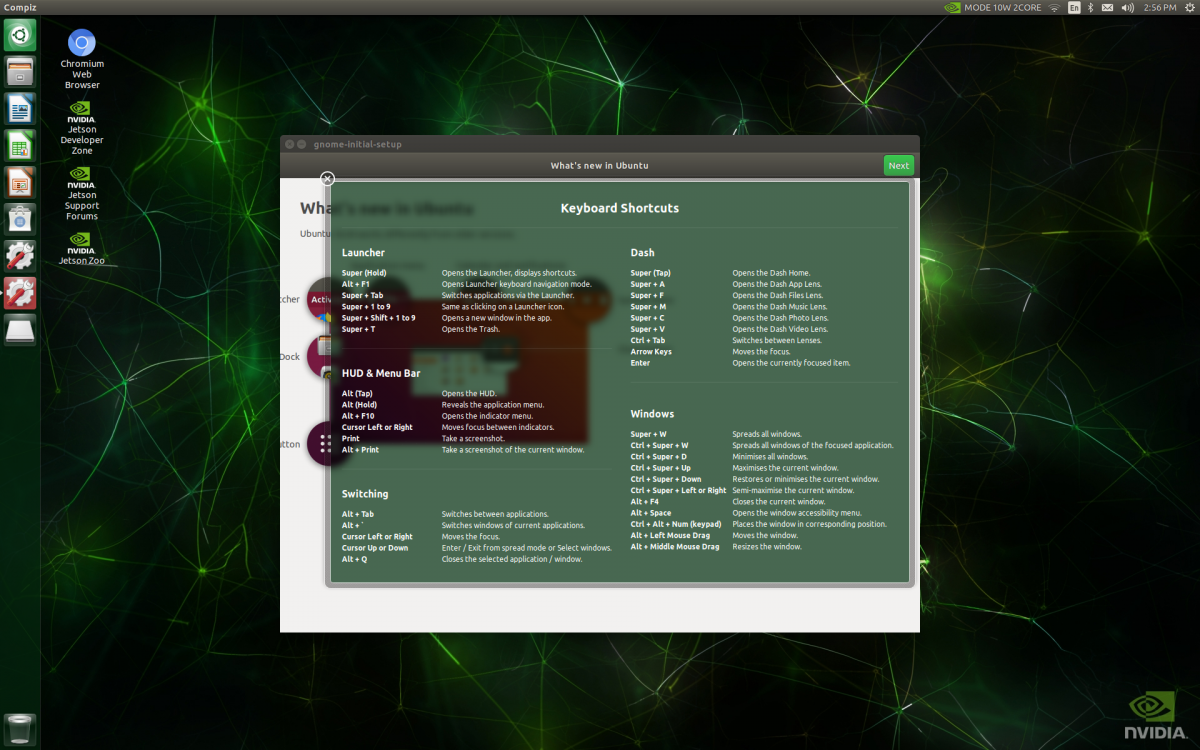
\includegraphics[width=0.7\textwidth ]{Bilder/jetson_booted_screen.png}
    \caption{Jetson Orin Nano Developer Kit - Desktop}
\end{figure}
\par \bigskip 

Führen Sie folgende Befehle aus. 
\begin{lstlisting}[language=bash]
sudo apt update
sudo apt upgrade
\end{lstlisting}
\clearpage

\section{Nächste Schritte}
\subsection{Sich zurechtfinden}

Lesen Sie \textcolor{blue}{\href{https://developer.nvidia.com/embedded/learn/jetson-orin-nano-devkit-user-guide/index.html}{das Benutzerhandbuch des Jetson Orin Nano Developer Kits}}, 
das Folgendes beinhaltet:
\begin{itemize}
    \item Viele weitere Details zur Hardware des Developer Kits
    \item Eine Übersicht über NVIDIA JetPack und Möglichkeiten, das Developer Kit zu flashen
    \item Besuchen Sie die \textcolor{blue}{\href{https://developer.nvidia.com/embedded-computing}{NVIDIA Jetson Developer-Website}} 
    für Zugriff auf alle Informationen zur Jetson-Plattform.
    \item Stellen Sie Fragen oder teilen Sie ein Projekt im \textcolor{blue}{\href{https://forums.developer.nvidia.com/c/agx-autonomous-machines/jetson-embedded-systems/70}{NVIDIA Jetson Forum}}.
\end{itemize}
\subsection{Benutzerdefinierte vorab konfigurierte SD-Karten-Abbilder}
Folgen Sie dem \textcolor{blue}{\href{https://nvidia-ai-iot.github.io/jetson_isaac_ros_visual_slam_tutorial/}{Jetson Isaac ROS Visual SLAM Tutorial}}, das Sie anleitet:
\begin{itemize}
    \item Richten Sie Ihr Jetson Orin Nano Developer Kit mit einer Intel RealSense Kamera ein, um die erstklassige VSLAM-Bibliothek schnell zu testen
    \item Mit einem vorab konfigurierten \textcolor{blue}{\href{https://nvidia-ai-iot.github.io/jetson_isaac_ros_visual_slam_tutorial/}{SD-Karten-Image}}, 
    das einen Großteil des Einrichtungsprozesses vereinfacht
\end{itemize}
\subsection{Quellen:}
\begin{itemize}
    \item \textcolor{blue}{\href{https://developer.nvidia.com/embedded/learn/getting-started-jetson}{Nvidia}}
\end{itemize}
\subsection{Weitere hilfreiche Quelle:}
\begin{itemize}
    \item \textcolor{blue}{\href{https://youtu.be/km0yT99eVTY?feature=shared}{Jetson Nano - Intro, Setup and Demo}}
    \item \textcolor{blue}{\href{https://youtu.be/Ucg5Zqm9ZMk?feature=shared}{NVIDIA SDK Manager Tutorial: Installing Jetson Software Explained}}
    \item \textcolor{blue}{\href{https://youtu.be/FX2exKW_20E?feature=shared}{Nvidia Jetson Orin Nano Unboxing und SSD Flash Install With SDK Manager}}
\end{itemize}

\end{document}